% !Mode:: "TeX:UTF-8"
% Translator: Shenjian Zhao
\chapter{前言}
\label{chap:introduction}
远在古希腊时期,发明家就梦想着创造能自主思考的机器。
神话人物皮格马利翁(Pygmalion)、代达罗斯(Daedalus)和赫淮斯托斯(Hephaestus)可以被看作传说中的发明家,而加拉蒂亚(Galatea)、塔洛斯(Talos)和潘多拉(Pandora)则可以被视为人造生命\citep{Ovid-Martin-2004,Sparkes-1996,Tandy-1997}。

当人类第一次构思可编程计算机时,就已经在思考计算机能否变得智能(尽管这距造出第一台计算机还有一百多年)\citep{Lovelace-1842}。
如今,\firstall{AI}已经成为一个具有众多实际应用和活跃研究课题的领域,并且正在蓬勃发展。
我们期望通过智能软件自动地处理常规劳动、理解语音或图像、帮助医学诊断和支持基础科学研究。

在\gls{AI}的早期,那些对人类智力来说非常困难、但对计算机来说相对简单的问题得到迅速解决,比如,那些可以通过一系列形式化的数学规则来描述的问题。
\gls{AI}的真正挑战在于解决那些对人来说很容易执行、但很难形式化描述的任务,如识别人们所说的话或图像中的脸。对于这些问题,我们人类往往可以凭借直觉轻易地解决。


针对这些比较直观的问题,本书讨论一种解决方案。
该方案可以让计算机从经验中学习,并根据层次化的概念体系来理解世界,而每个概念则通过与某些相对简单的概念之间的关系来定义。
让计算机从经验获取知识,可以避免由人类来给计算机形式化地指定它需要的所有知识。
层次化的概念让计算机构建较简单的概念来学习复杂概念。
如果绘制出这些概念如何建立在彼此之上的图,我们将得到一张``深''(层次很多)的图。
基于这个原因,我们称这种方法为~\glssymbol{AI}\firstgls{DL}。

% -- 1 --

\glssymbol{AI}~许多早期的成功发生在相对朴素且形式化的环境中, 而且不要求计算机具备很多关于世界的知识。
例如,IBM的深蓝(Deep Blue)国际象棋系统在1997年击败了世界冠军\ENNAME{Garry Kasparov}\citep{Hsu-2002}。
显然国际象棋是一个非常简单的领域,因为它仅含有64个位置并只能以严格限制的方式移动32个棋子。
设计一种成功的国际象棋策略是巨大的成就,但向计算机描述棋子及其允许的走法并不是挑战的困难所在。
国际象棋完全可以由一个非常简短的、完全形式化的规则列表来描述,并可以容易地由程序员事先准备好。

讽刺的是,抽象和形式化的任务对人类而言是最困难的脑力任务之一,但对计算机而言却属于最容易的。
计算机早就能够打败人类最好的象棋选手,但直到最近计算机才在识别对象或语音任务中达到人类平均水平。
一个人的日常生活需要关于世界的巨量知识。
很多这方面的知识是主观的、直观的,因此很难通过形式化的方式表达清楚。
计算机需要获取同样的知识才能表现出智能。
\gls{AI}的一个关键挑战就是如何将这些非形式化的知识传达给计算机。

一些\gls{AI}项目力求将关于世界的知识用形式化的语言进行硬编码(hard-code)。
计算机可以使用逻辑推理规则来自动地理解这些形式化语言中的声明。
这就是众所周知的\gls{AI}的\firstgls{knowledge_base}方法。
然而,这些项目最终都没有取得重大的成功。
其中最著名的项目是Cyc \citep{Lenat-Guha-1989}。
Cyc包括一个\gls{inference}引擎和一个使用CycL语言描述的声明数据库。
这些声明是由人类监督者输入的。
这是一个笨拙的过程。
人们设法设计出足够复杂的形式化规则来精确地描述世界。
例如,Cyc不能理解一个关于名为~\ENNAME{Fred}~的人在早上剃须的故事\citep{Linde-1992}。
它的推理引擎检测到故事中的不一致性:它知道人没有电气零件,但由于~\ENNAME{Fred}~正拿着一个电动剃须刀,它认为实体
``正在剃须的Fred''\,(``FredWhileShaving'')含有电气部件。
因此它产生了这样的疑问——\ENNAME{Fred}~在刮胡子的时候是否仍然是一个人。

依靠硬编码的知识体系面对的困难表明,\glssymbol{AI}~系统需要具备自己获取知识的能力,即从原始数据中提取模式的能力。
这种能力被称为\firstgls{ML}。
引入\gls{ML}使计算机能够解决涉及现实世界知识的问题,并能作出看似主观的决策。
比如,一个被称为\firstgls{logistic_regression}的简单\gls{ML}算法可以决定是否建议剖腹产\citep{Mor-Yosef-et-al-1990}。
而同样是简单\gls{ML}算法的\firstgls{naive_bayes}则可以区分垃圾电子邮件和合法电子邮件。

% -- 2 --

这些简单的\gls{ML}算法的性能在很大程度上依赖于给定数据的\firstgls{representation}。
例如,当\gls{logistic_regression}被用于判断产妇是否适合剖腹产时,\glssymbol{AI}~系统不会直接检查患者。
相反,医生需要告诉系统几条相关的信息,诸如是否存在子宫疤痕。
表示患者的每条信息被称为一个特征。
\gls{logistic_regression}学习病人的这些特征如何与各种结果相关联。
然而,它丝毫不能影响该特征定义的方式。
如果将病人的MRI扫描作为\gls{logistic_regression}的输入,而不是医生正式的报告,它将无法作出有用的预测。
MRI扫描的单一像素与分娩过程中并发症之间的相关性微乎其微。

在整个计算机科学乃至日常生活中,对\gls{representation}的依赖都是一个普遍现象。
在计算机科学中,如果数据集合被精巧地结构化并被智能地索引,那么诸如搜索之类的操作的处理速度就可以成指数级地加快。
人们可以很容易地在阿拉伯数字的\gls{representation}下进行算术运算,但在罗马数字的\gls{representation}下运算会比较耗时。
因此,毫不奇怪,\gls{representation}的选择会对\gls{ML}算法的性能产生巨大的影响。
\figref{fig:chap1_polar}展示了一个简单的可视化例子。

\begin{figure}[!htb]
\ifOpenSource
\centerline{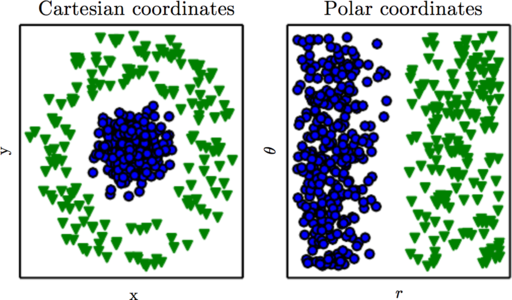
\includegraphics[scale=0.5]{images/1.png}}
\else
\centerline{\includegraphics{Chapter1/figures/polar_color}}
\fi
\caption{不同表示的例子:假设我们想在散点图中画一条线来分隔两类数据。
在左图,我们使用笛卡尔坐标表示数据,这个任务是不可能的。 
右图中,我们用极坐标表示数据,可以用垂直线简单地解决这个任务。(与David Warde-Farley合作画出此图。)}
\label{fig:chap1_polar}
\end{figure}

许多\gls{AI}任务都可以通过以下方式解决:先提取一个合适的特征集,然后将这些特征提供给简单的\gls{ML}算法。
例如,对于通过声音鉴别说话者的任务来说,一个有用的特征是对其声道大小的估计。
这个特征为判断说话者是男性、女性还是儿童提供了有力线索。

然而,对于许多任务来说,我们很难知道应该提取哪些特征。
例如,假设我们想编写一个程序来检测照片中的车。
我们知道,汽车有轮子,所以我们可能会想用车轮的存在与否作为特征。
不幸的是,我们难以准确地根据像素值来描述车轮看上去像什么。
虽然车轮具有简单的几何形状,但它的图像可能会因场景而异,如落在车轮上的阴影、太阳照亮的车轮的金属零件、汽车的挡泥板或者遮挡的车轮一部分的前景物体等等。

% -- 3 --

解决这个问题的途径之一是使用\gls{ML}来发掘\gls{representation}本身,而不仅仅把\gls{representation}映射到输出。
这种方法我们称之为\firstgls{representation_learning}。
学习到的\gls{representation}往往比手动设计的\gls{representation}表现得更好。
并且它们只需最少的人工干预,就能让\glssymbol{AI}系统迅速适应新的任务。
\gls{representation_learning}算法只需几分钟就可以为简单的任务发现一个很好的特征集,对于复杂任务则需要几小时到几个月。
手动为一个复杂的任务设计特征需要耗费大量的人工时间和精力;甚至需要花费整个社群研究人员几十年的时间。

\gls{representation_learning}算法的典型例子是\firstgls{AE}。
\gls{AE}由一个\firstgls{encoder}函数和一个\firstgls{decoder}函数组合而成。
\gls{encoder}函数将输入数据转换为一种不同的\gls{representation},而\gls{decoder}函数则将这个新的\gls{representation}转换到原来的形式。
我们期望当输入数据经过\gls{encoder}和\gls{decoder}之后尽可能多地保留信息,同时希望新的\gls{representation}有各种好的特性,
这也是\gls{AE}的训练目标。
为了实现不同的特性,我们可以设计不同形式的\gls{AE}。

当设计特征或设计用于学习特征的算法时,我们的目标通常是分离出能解释观察数据的\firstgls{factors_of_variation}。
在此背景下,``因素''这个词仅指代影响的不同来源;因素通常不是乘性组合。
这些因素通常是不能被直接观察到的量。
相反,它们可能是现实世界中观察不到的物体或者不可观测的力,但会影响可观测的量。
为了对观察到的数据提供有用的简化解释或推断其原因,它们还可能以概念的形式存在于人类的思维中。
它们可以被看作数据的概念或者抽象,帮助我们了解这些数据的丰富多样性。
当分析语音记录时,\gls{factors_of_variation}包括说话者的年龄、性别、他们的口音和他们正在说的词语。
当分析汽车的图像时,\gls{factors_of_variation}包括汽车的位置、它的颜色、太阳的角度和亮度。

% -- 4 --

在许多现实的\gls{AI}应用中,困难主要源于多个\gls{factors_of_variation}同时影响着我们能够观察到的每一个数据。
比如,在一张包含红色汽车的图片中,其单个像素在夜间可能会非常接近黑色。
汽车轮廓的形状取决于视角。
大多数应用需要我们\emph{理清}\gls{factors_of_variation}并忽略我们不关心的因素。

显然,从原始数据中提取如此高层次、抽象的特征是非常困难的。
许多诸如说话口音这样的\gls{factors_of_variation},只能通过对数据进行复杂的、接近人类水平的理解来辨识。
这几乎与获得原问题的\gls{representation}一样困难,因此,乍一看,\gls{representation_learning}似乎并不能帮助我们。

\firstgls{DL}通过其他较简单的\gls{representation}来表达复杂\gls{representation},解决了\gls{representation_learning}中的核心问题。

\begin{figure}[!htb]
\ifOpenSource
\centerline{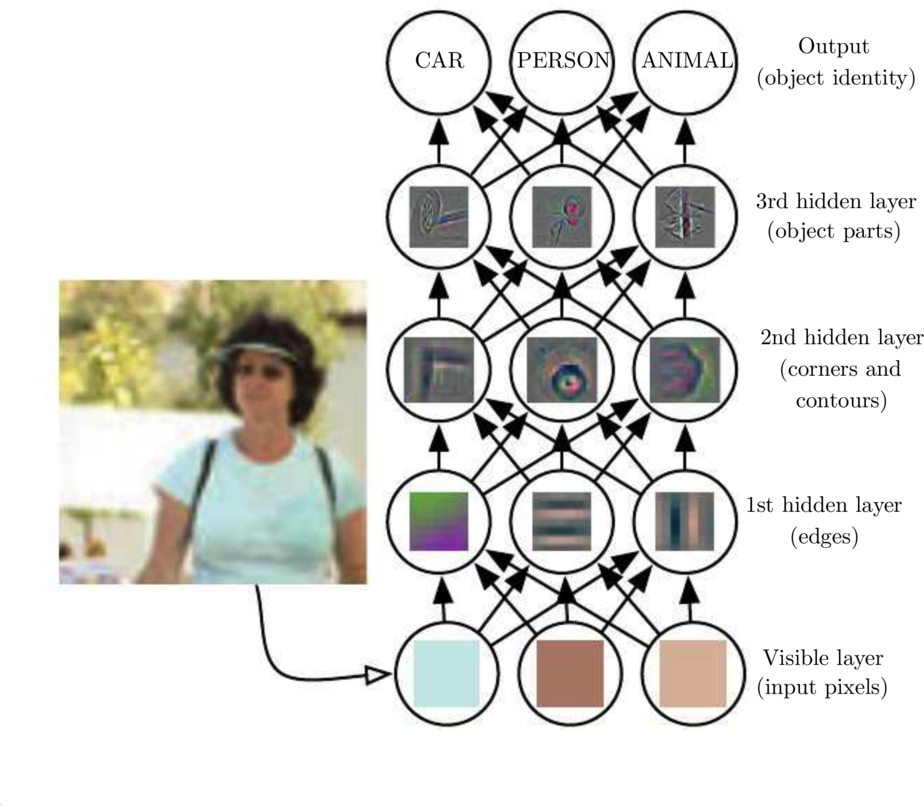
\includegraphics[scale=0.5]{images/2.png}}
\else
\centerline{\includegraphics{Chapter1/figures/deep_learning}}
\fi
\caption{深度学习模型的示意图。 计算机难以理解原始感观输入数据的含义,如表示为像素值集合的图像。
将一组像素映射到对象标识的函数非常复杂。
如果直接处理,学习或评估此映射似乎是不可能的。
深度学习将所需的复杂映射分解为一系列嵌套的简单映射(每个由模型的不同层描述)来解决这一难题。
输入展示在\firstgls{visible_layer},这样命名的原因是因为它包含我们能观察到的变量。
然后是一系列从图像中提取越来越多抽象特征的\firstgls{hidden_layer}。
因为它们的值不在数据中给出,所以将这些层称为``隐藏''; 模型必须确定哪些概念有利于解释观察数据中的关系。
这里的图像是每个\gls{hidden_unit}表示的特征的可视化。
给定像素,第一层可以轻易地通过比较相邻像素的亮度来识别边缘。
有了第一\gls{hidden_layer}描述的边缘,第二\gls{hidden_layer}可以容易地搜索可识别为角和扩展轮廓的边集合。
给定第二\gls{hidden_layer}中关于角和轮廓的图像描述,第三\gls{hidden_layer}可以找到轮廓和角的特定集合来检测特定对象的整个部分。
最后,根据图像描述中包含的对象部分,可以识别图像中存在的对象。
经~\citet{Zeiler-Fergus-2014}许可转载此图。
}
\label{fig:chap1_deep_learning}
\end{figure}

\gls{DL}让计算机通过较简单概念构建复杂的概念。
\figref{fig:chap1_deep_learning}展示了\gls{DL}系统如何通过组合较简单的概念(例如转角和轮廓,它们转而由边线定义)来表示图像中人的概念。
\gls{DL}模型的典型例子是前馈深度网络或\firstall{MLP}。
\gls{MLP}仅仅是一个将一组输入值映射到输出值的数学函数。
该函数由许多较简单的函数复合而成。
我们可以认为不同数学函数的每一次应用都为输入提供了新的\gls{representation}。

学习数据的正确\gls{representation}的想法是解释\gls{DL}的一个视角。
另一个视角是深度促使计算机学习一个多步骤的计算机程序。
每一层\gls{representation}都可以被认为是并行执行另一组指令之后计算机的存储器状态。
更深的网络可以按顺序执行更多的指令。
顺序指令提供了极大的能力,因为后面的指令可以参考早期指令的结果。
从这个角度上看,在某层激活函数里,并非所有信息都蕴涵着解释输入的\gls{factors_of_variation}。
\gls{representation}还存储着状态信息,用于帮助程序理解输入。
这里的状态信息类似于传统计算机程序中的计数器或指针。
它与具体的输入内容无关,但有助于模型组织其处理过程。

% -- 6 --

目前主要有两种度量模型深度的方式。
第一种方式是基于评估架构所需执行的顺序指令的数目。
假设我们将模型表示为给定输入后,计算对应输出的流程图,则可以将这张流程图中的最长路径视为模型的深度。
正如两个使用不同语言编写的等价程序将具有不同的长度;相同的函数可以被绘制为具有不同深度的流程图,其深度取决于我们可以用来作为一个步骤的函数。
\figref{fig:chap1_language}说明了语言的选择如何给相同的架构两个不同的衡量。

\begin{figure}[!htb]
\ifOpenSource
\centerline{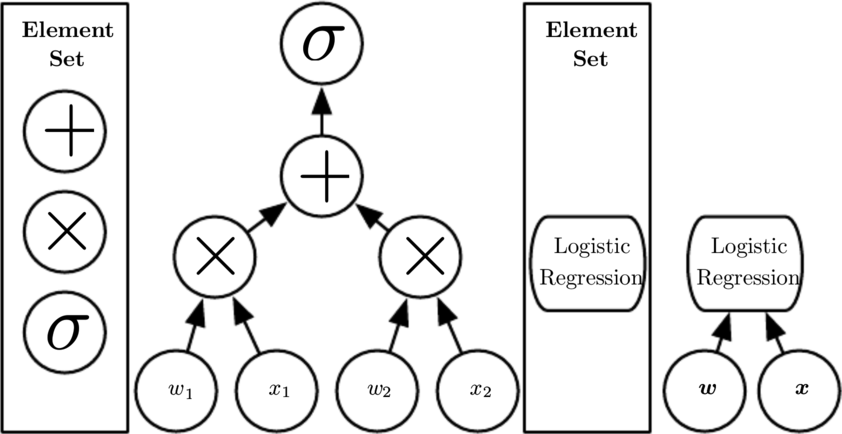
\includegraphics[scale=0.5]{images/3.png}}
\else
\centerline{\includegraphics{Chapter1/figures/language}}
\fi
\caption{将输入映射到输出的计算图表的示意图,其中每个节点执行一个操作。
深度是从输入到输出的最长路径的长度,但这取决于可能的计算步骤的定义。
这些图中所示的计算是\gls{logistic_regression}模型的输出,$\sigma(\Vw^T \Vx)$,其中$\sigma$是~\ENNAME{logistic sigmoid}~函数。
如果我们使用加法、乘法和~\ENNAME{logistic sigmoid}~作为我们计算机语言的元素,那么这个模型深度为三。
如果我们将\gls{logistic_regression}视为元素本身,那么这个模型深度为一。
}
\label{fig:chap1_language}
\end{figure}

另一种是在深度概率模型中使用的方法,它不是将计算图的深度视为模型深度,而是将描述概念彼此如何关联的图的深度视为模型深度。
在这种情况下,计算每个概念\gls{representation}的计算流程图的深度可能比概念本身的图更深。
这是因为系统对较简单概念的理解在给出更复杂概念的信息后可以进一步精细化。
例如,一个~\glssymbol{AI}~系统观察其中一只眼睛在阴影中的脸部图像时,它最初可能只看到一只眼睛。
但当检测到脸部的存在后,系统可以推断第二只眼睛也可能是存在的。
在这种情况下,概念的图仅包括两层(关于眼睛的层和关于脸的层),但如果我们细化每个概念的估计将需要额外的$n$次计算,即计算的图将包含$2n$层。

% -- 7 --

由于并不总是清楚计算图的深度或概率模型图的深度哪一个是最有意义的,并且由于不同的人选择不同的最小元素集来构建相应的图,因此就像计算机程序的长度不存在单一的正确值一样,架构的深度也不存在单一的正确值。
另外,也不存在模型多么深才能被修饰为``深''的共识。
但相比传统\gls{ML},\gls{DL}研究的模型涉及更多学到功能或学到概念的组合,这点毋庸置疑。

总之, 这本书的主题——\gls{DL}是通向\gls{AI}的途径之一。
具体来说,它是\gls{ML}的一种,一种能够使计算机系统从经验和数据中得到提高的技术。
我们坚信\gls{ML}可以构建出在复杂实际环境下运行的~\glssymbol{AI}~系统,并且是唯一切实可行的方法。
\gls{DL}是一种特定类型的\gls{ML},具有强大的能力和灵活性,它将大千世界\gls{representation}为嵌套的层次概念体系
(由较简单概念间的联系定义复杂概念、从一般抽象概括到高级抽象表示)。
\figref{fig:chap1_venn}说明了这些不同的~\glssymbol{AI}~学科之间的关系。\figref{fig:chap1_which_part_learned}展示了每个学科如何工作的高层次原理。

\begin{figure}[!hbt]
\ifOpenSource
\centerline{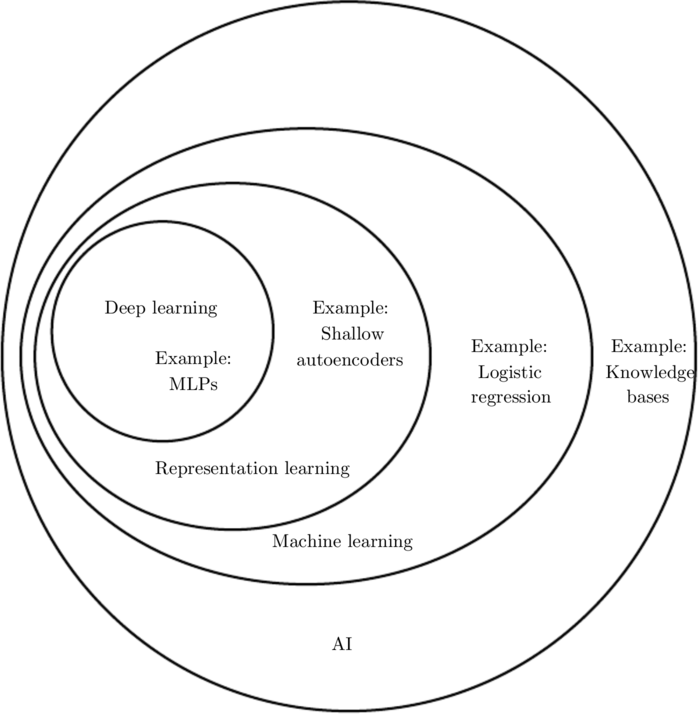
\includegraphics[scale=0.5]{images/4.png}}
\else
\centerline{\includegraphics[width=0.65\textwidth]{Chapter1/figures/venn}}
\fi
\caption{维恩图展示了深度学习是一种表示学习,也是一种机器学习,可以用于许多(但不是全部)\glssymbol{AI}~方法。
维恩图的每个部分包括一个~\glssymbol{AI}~技术的示例。
}
\label{fig:chap1_venn}
\end{figure}

\begin{figure}[!htb]
\ifOpenSource
\centerline{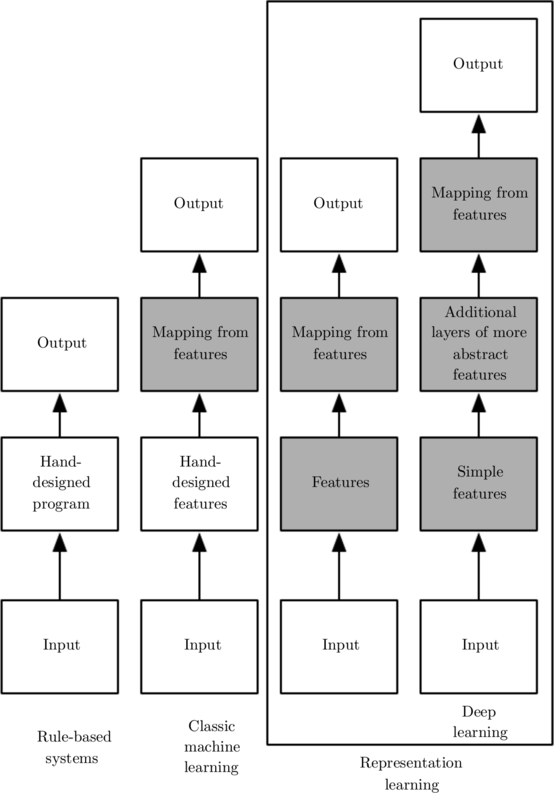
\includegraphics[scale=0.5]{images/5.png}}
\else
\centerline{\includegraphics{Chapter1/figures/which_part_learned}}
\fi
\caption{流程图展示了~\glssymbol{AI}~系统的不同部分如何在不同的~\glssymbol{AI}~学科中彼此相关。
阴影框表示能从数据中学习的组件。}
\label{fig:chap1_which_part_learned}
\end{figure}

\section{本书面向的读者}
\label{sec:who_should_read_this_book}

这本书对各类读者都有一定用处,但我们主要是为两类受众对象而写的。
其中一类受众对象是学习\gls{ML}的大学生(本科或研究生),包括那些已经开始职业生涯的\gls{DL}和\gls{AI}研究者。
另一类受众对象是没有\gls{ML}或统计背景但希望能快速地掌握这方面知识并在他们的产品或平台中使用\gls{DL}的软件工程师。
\gls{DL}在许多软件领域都已被证明是有用的,包括计算机视觉、语音和音频处理、自然语言处理、机器人技术、生物信息学和化学、电子游戏、搜索引擎、网络广告和金融。

\begin{figure}[!htb]
\ifOpenSource
\centerline{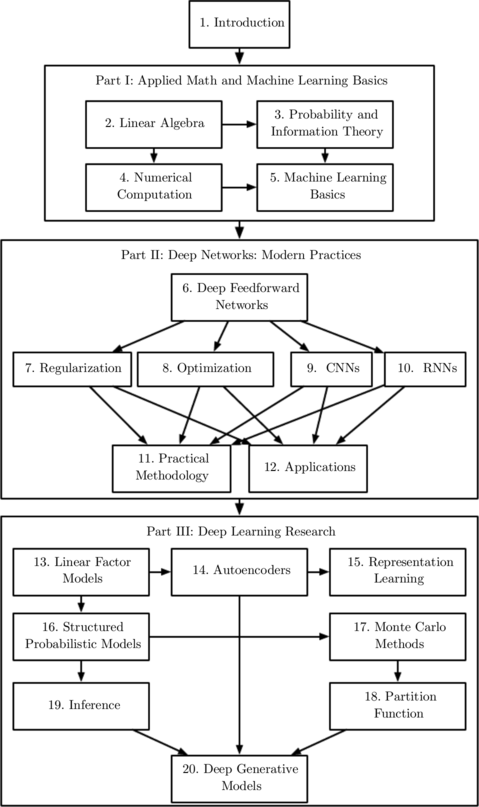
\includegraphics[scale=0.5]{images/6.png}}
\else
\centerline{\includegraphics[width=0.65\textwidth]{Chapter1/figures/dependency}}
\fi
\caption{本书的高层组织。
从一章到另一章的箭头表示前一章是理解后一章的必备内容。}
\label{fig:chap1_dependency}
\end{figure}

% -- 8 --

为了最好地服务各类读者,我们将本书组织为三个部分。
第一部分介绍基本的数学工具和\gls{ML}的概念。
第二部分介绍最成熟的\gls{DL}算法,这些技术基本上已经得到解决。
第三部分讨论某些具有展望性的想法,它们被广泛地认为是\gls{DL}未来的研究重点。

读者可以随意跳过不感兴趣或与自己背景不相关的部分。
熟悉线性代数、概率和基本\gls{ML}概念的读者可以跳过第一部分,例如,当读者只是想实现一个能工作的系统则不需要阅读超出第二部分的内容。
为了帮助读者选择章节,\figref{fig:chap1_dependency}展示了这本书的高层组织结构的流程图。

% -- 10 --

我们假设所有读者都具备计算机科学背景。
也假设读者熟悉编程,并且对计算的性能问题、复杂性理论、入门级微积分和一些图论术语有基本的了解。
% 
\section{深度学习的历史趋势}
\label{sec:historical_trends_in_deep_learning}
通过历史背景了解\gls{DL}是最简单的方式。
这里我们仅指出\gls{DL}的几个关键趋势,而不是提供其详细的历史:
\begin{itemize}
 \item \gls{DL}有着悠久而丰富的历史,但随着许多不同哲学观点的渐渐消逝,与之对应的名称也渐渐尘封。
 \item 随着可用的训练数据量不断增加,\gls{DL}变得更加有用。
 \item 随着时间的推移,针对\gls{DL}的计算机软硬件基础设施都有所改善,\gls{DL}模型的规模也随之增长。
 \item 随着时间的推移,\gls{DL}已经解决日益复杂的应用,并且精度不断提高。
\end{itemize}

\subsection{神经网络的众多名称和命运变迁}
\label{sec:the_many_names_and_changing_fortunes_of_neural_networks}

我们期待这本书的许多读者都听说过\gls{DL}这一激动人心的新技术,并对一本书提及一个新兴领域的``历史''而感到惊讶。
事实上,\gls{DL}的历史可以追溯到20世纪40年代。
\gls{DL}\emph{看似}是一个全新的领域,只不过因为在目前流行的前几年它是相对冷门的,同时也因为它被赋予了许多不同的名称(其中大部分已经不再使用),最近才成为众所周知的``\gls{DL}''。
这个领域已经更换了很多名称,它反映了不同的研究人员和不同观点的影响。

全面地讲述\gls{DL}的历史超出了本书的范围。
然而,一些基本的背景对理解\gls{DL}是有用的。
一般来说,目前为止\gls{DL}已经经历了三次发展浪潮:20世纪40年代到60年代\gls{DL}的雏形出现在\firstgls{cybernetics}中,20世纪80年代到90年代\gls{DL}表现为\firstgls{connectionism},直到2006年,才真正以\gls{DL}之名复兴。
\figref{fig:chap1_cybernetics_connectionism_ngrams_color}给出了定量的展示。

\begin{figure}[!htb]
\ifOpenSource
\centerline{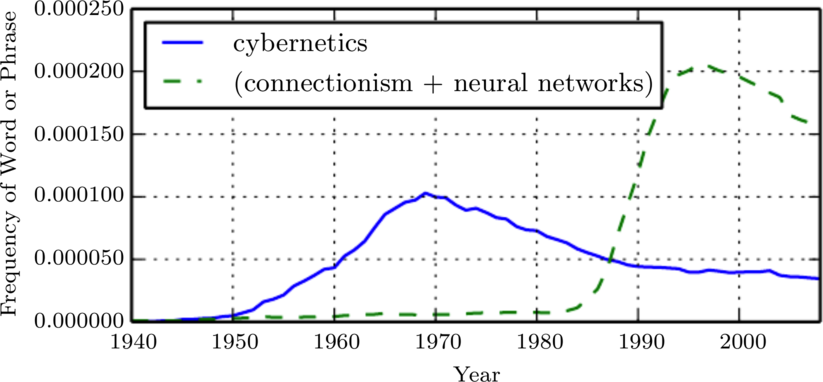
\includegraphics[scale=0.5]{images/7.png}}
\else
\centerline{\includegraphics{Chapter1/figures/cybernetics_connectionism_ngrams_color}}
\fi
\caption{根据Google图书中短语``\gls{cybernetics}''、``\gls{connectionism}''或``\gls{NN}''频率衡量的\gls{ANN}研究的历史浪潮(图中展示了三次浪潮的前两次,第三次最近才出现)。
第一次浪潮开始于20世纪40年代到20世纪60年代的\gls{cybernetics},随着生物学习理论的发展\citep{McCulloch-Pitts-1943,Hebb-1949}
和第一个模型的实现(如感知机~\citep{Rosenblatt-1958}) ,能实现单个神经元的训练。
第二次浪潮开始于1980-1995年间的\gls{connectionism}方法,可以使用反向传播\citep{Rumelhart-et-al-1986a} 训练具有一两个\gls{hidden_layer}的神经网络。
当前第三次浪潮,也就是深度学习,大约始于2006年\citep{Hinton-et-al-2006,Bengio-et-al-2007,Ranzato-et-al-2007a},并且现在在2016年以书的形式出现。
另外两次浪潮类似地出现在书中的时间比相应的科学活动晚得多。
}
\label{fig:chap1_cybernetics_connectionism_ngrams_color}
\end{figure}

% -- 12 --

我们今天知道的一些最早的学习算法,是旨在模拟生物学习的计算模型,即大脑怎样学习或为什么能学习的模型。
其结果是\gls{DL}以\firstall{ANN}之名而淡去。
彼时,\gls{DL}模型被认为是受生物大脑(无论人类大脑或其他动物的大脑)所启发而设计出来的系统。
尽管有些\gls{ML}的\gls{NN}有时被用来理解大脑功能\citep{Hinton-Shallice-1991},但它们一般都没有被设计成生物功能的真实模型。
\gls{DL}的神经观点受两个主要思想启发。
一个想法是大脑作为例子证明智能行为是可能的,因此,概念上,建立智能的直接途径是逆向大脑背后的计算原理,并复制其功能。
另一种看法是,理解大脑和人类智能背后的原理也非常有趣,因此\gls{ML}模型除了解决工程应用的能力, 如果能让人类对这些基本的科学问题有进一步的认识也将会很有用。

% -- 13 --
  
现代术语``\gls{DL}''超越了目前\gls{ML}模型的神经科学观点。
它诉诸于学习\emph{多层次组合}这一更普遍的原理,这一原理也可以应用于那些并非受神经科学启发的\gls{ML}框架。
 
 
现代\gls{DL}的最早前身是从神经科学的角度出发的简单线性模型。
这些模型被设计为使用一组$\Sn$个输入$\Sx_1, \dots ,\Sx_n$并将它们与一个输出$\Sy$相关联。 
这些模型希望学习一组权重$\Sw_1, \dots, \Sw_n $,并计算它们的输出$f(\Vx, \Vw) = \Sx_1 \Sw_1 + \dots + \Sx_n \Sw_n$。
如\figref{fig:chap1_cybernetics_connectionism_ngrams_color}所示,这第一波\gls{NN}研究浪潮被称为\gls{cybernetics}。

\ENNAME{McCulloch-Pitts}~神经元\citep{McCulloch-Pitts-1943}是脑功能的早期模型。
该线性模型通过检验函数$f(\Vx,\Vw)$的正负来识别两种不同类别的输入。
显然,模型的权重需要正确设置后才能使模型的输出对应于期望的类别。
这些权重可以由操作人员设定。
在20世纪50年代,感知机\citep{Rosenblatt-1958,Rosenblatt-1962}成为第一个能根据每个类别的输入\gls{example}来学习权重的模型。
约在同一时期,\textbf{自适应线性单元}(adaptive linear element, ADALINE)简单地返回函数$f(\Vx)$本身的值来预测一个实数\citep{Widrow-Hoff-1960},并且它还可以学习从数据预测这些数。

这些简单的学习算法大大影响了\gls{ML}的现代景象。
用于调节ADALINE权重的训练算法是被称为\firstgls{SGD}的一种特例。
稍加改进后的\gls{SGD}算法仍然是当今\gls{DL}的主要训练算法。

基于感知机和ADALINE中使用的函数$f(\Vx, \Vw)$的模型被称为\firstgls{linear_model}。
尽管在许多情况下,这些模型以不同于原始模型的方式进行\emph{训练},但仍是目前最广泛使用的\gls{ML}模型。

\gls{linear_model}有很多局限性。
最著名的是,它们无法学习异或(XOR)函数,即$f([0,1], \Vw) = 1$和$f([1,0], \Vw)=1$,但$f([1,1], \Vw)=0$和$f([0,0],\Vw)= 0$。
观察到\gls{linear_model}这个缺陷的批评者对受生物学启发的学习普遍地产生了抵触\citep{Minsky-Papert-1969}。
这导致了\gls{NN}热潮的第一次大衰退。

现在,神经科学被视为\gls{DL}研究的一个重要灵感来源,但它已不再是该领域的主要指导。

% -- 14 --

如今神经科学在\gls{DL}研究中的作用被削弱,主要原因是我们根本没有足够的关于大脑的信息来作为指导去使用它。
要获得对被大脑实际使用算法的深刻理解,我们需要有能力同时监测(至少是)数千相连神经元的活动。
我们不能够做到这一点,所以我们甚至连大脑最简单、最深入研究的部分都还远远没有理解\citep{Olshausen-Field-2005}。

神经科学已经给了我们依靠单一\gls{DL}算法解决许多不同任务的理由。
神经学家们发现,如果将雪貂的大脑重新连接,使视觉信号传送到听觉区域,它们可以学会用大脑的听觉处理区域去``看''~\citep{Von-Melchner-et-al-2000}。
这暗示着大多数哺乳动物的大脑能够使用单一的算法就可以解决其大脑可以解决的大部分不同任务。
在这个假设之前,\gls{ML}研究是比较分散的,研究人员在不同的社群研究自然语言处理、计算机视觉、运动规划和语音识别。
如今,这些应用社群仍然是独立的,但是对于\gls{DL}研究团体来说,同时研究许多或甚至所有这些应用领域是很常见的。

我们能够从神经科学得到一些粗略的指南。
仅通过计算单元之间的相互作用而变得智能的基本思想是受大脑启发的。
新认知机\citep{Fukushima-1980}受哺乳动物视觉系统的结构启发,引入了一个处理图片的强大模型架构,它后来成为了现代卷积网络的基础\citep{LeCun-et-al-1998b}(我们将会在\secref{sec:the_neuroscientific_basis_for_convolutional_networks}看到)。
目前大多数\gls{NN}是基于一个称为\firstgls{ReLU}的神经单元模型。
原始认知机\citep{Fukushima-1975}受我们关于大脑功能知识的启发, 引入了一个更复杂的版本。
简化的现代版通过吸收来自不同观点的思想而形成,\citet{Nair-Hinton-2010}和~\citet{Glorot-et-al-2011a}援引神经科学作为影响,\citet{Jarrett-et-al-2009}援引更多面向工程的影响。
虽然神经科学是灵感的重要来源,但它不需要被视为刚性指导。
我们知道,真实的神经元计算着与现代\gls{ReLU}非常不同的函数,但更接近真实神经网络的系统并没有导致\gls{ML}性能的提升。
此外,虽然神经科学已经成功地启发了一些\gls{NN}\emph{架构},但我们对用于神经科学的生物学习还没有足够多的了解,因此也就不能为训练这些架构用的\emph{学习算法}提供太多的借鉴。


媒体报道经常强调\gls{DL}与大脑的相似性。
的确,\gls{DL}研究者比其他\gls{ML}领域(如核方法或贝叶斯统计)的研究者更可能地引用大脑作为影响,但是大家不应该认为\gls{DL}在尝试模拟大脑。
现代\gls{DL}从许多领域获取灵感,特别是应用数学的基本内容如线性代数、概率论、信息论和数值优化。
尽管一些\gls{DL}的研究人员引用神经科学作为灵感的重要来源,然而其他学者完全不关心神经科学。

% -- 15 --

值得注意的是,了解大脑是如何在算法层面上工作的尝试确实存在且发展良好。
这项尝试主要被称为``计算神经科学'',并且是独立于\gls{DL}的领域。
研究人员在两个领域之间来回研究是很常见的。
\gls{DL}领域主要关注如何构建计算机系统,从而成功解决需要智能才能解决的任务,而计算神经科学领域主要关注构建大脑如何真实工作的比较精确的模型。

在20世纪80年代,神经网络研究的第二次浪潮在很大程度上是伴随一个被称为\firstgls{connectionism}或\textbf{并行分布处理}( parallel distributed processing)潮流而出现的\citep{Rumelhart-et-al-1986c,McClelland-et-al-1995}。
\gls{connectionism}是在认知科学的背景下出现的。
认知科学是理解思维的跨学科途径,即它融合多个不同的分析层次。
在20世纪80年代初期,大多数认知科学家研究符号推理模型。
尽管这很流行,但符号模型很难解释大脑如何真正使用神经元实现推理功能。 
\gls{connectionism}者开始研究真正基于神经系统实现的认知模型\citep{Touretzky-Minton-1985},其中很多复苏的想法可以追溯到心理学家~\ENNAME{Donald Hebb}~在20世纪40年代的工作\citep{Hebb-1949}。

\gls{connectionism}的中心思想是,当网络将大量简单的计算单元连接在一起时可以实现智能行为。
这种见解同样适用于生物神经系统中的神经元,因为它和计算模型中\gls{hidden_unit}起着类似的作用。

在上世纪80年代的\gls{connectionism}期间形成的几个关键概念在今天的\gls{DL}中仍然是非常重要的。

其中一个概念是\firstgls{distributed_representation}\citep{Hinton-et-al-1986}。
其思想是:系统的每一个输入都应该由多个特征\gls{representation},并且每一个特征都应该参与到多个可能输入的\gls{representation}。
例如,假设我们有一个能够识别红色、绿色、或蓝色的汽车、卡车和鸟类的视觉系统,
\gls{representation}这些输入的其中一个方法是将九个可能的组合:红卡车,红汽车,红鸟,绿卡车等等使用单独的神经元或\gls{hidden_unit}激活。
这需要九个不同的神经元,并且每个神经必须独立地学习颜色和对象身份的概念。
改善这种情况的方法之一是使用\gls{distributed_representation},即用三个神经元描述颜色,三个神经元描述对象身份。 
这仅仅需要6个神经元而不是9个,并且描述红色的神经元能够从汽车、卡车和鸟类的图像中学习红色,而不仅仅是从一个特定类别的图像中学习。 
\gls{distributed_representation}的概念是本书的核心,我们将在\chapref{chap:representation_learning}中更加详细地描述。

% -- 16 --

\gls{connectionism}潮流的另一个重要成就是反向传播在训练具有内部\gls{representation}的深度\gls{NN}中的成功使用以及反向传播算法的普及\citep{Rumelhart-et-al-1986a,LeCun-1987}。
这个算法虽然曾黯然失色不再流行,但截至写书之时,它仍是训练深度模型的主导方法。% ??

在20世纪90年代,研究人员在使用\gls{NN}进行序列建模的方面取得了重要进展。
\citet{Hochreiter-1991}和~\citet{Bengio-et-al-1994}指出了对长序列进行建模的一些根本性数学难题,这将在\secref{sec:the_challenge_of_long_term_dependencies}中描述。
\citet{Hochreiter-Schmidhuber-1997}引入\firstall{LSTM}网络来解决这些难题。
如今,\glssymbol{LSTM}~在许多序列建模任务中广泛应用,包括Google的许多自然语言处理任务。

\gls{NN}研究的第二次浪潮一直持续到上世纪90年代中期。
基于\gls{NN}和其他\glssymbol{AI}技术的创业公司开始寻求投资,其做法野心勃勃但不切实际。
当\glssymbol{AI}研究不能实现这些不合理的期望时,投资者感到失望。
同时,\gls{ML}的其他领域取得了进步。
比如,核方法\citep{Boser-et-al-1992,Cortes-Vapnik-1995,Scholkopf-et-al-1999}和图模型\citep{Jordan-1998}都在很多重要任务上实现了很好的效果。
这两个因素导致了\gls{NN}热潮的第二次衰退,并一直持续到2007年。

在此期间,\gls{NN}继续在某些任务上获得令人印象深刻的表现\citep{LeCun-et-al-1998b,Bengio-et-al-2001}。
加拿大高级研究所(CIFAR)通过其神经计算和自适应感知(NCAP)研究计划帮助维持\gls{NN}研究。
该计划联合了分别由~\ENNAME{Geoffrey Hinton}、\ENNAME{Yoshua Bengio}和~\ENNAME{Yann LeCun}~领导的多伦多大学、蒙特利尔大学和纽约大学的\gls{ML}研究小组。
这个多学科的CIFAR NCAP研究计划还囊括了神经科学家、人类和计算机视觉专家。

% -- 17 --

在那个时候,人们普遍认为深度网络是难以训练的。
现在我们知道,20世纪80年代就存在的算法能工作得非常好,但是直到在2006年前后都没有体现出来。
这可能仅仅由于其计算代价太高,而以当时可用的硬件难以进行足够的实验。

神经网络研究的第三次浪潮始于2006年的突破。
\ENNAME{Geoffrey Hinton}~表明名为\gls{DBN}的\gls{NN}可以使用一种称为贪婪逐层预训练的策略来有效地训练\citep{Hinton-et-al-2006},我们将在\secref{sec:greedy_layer_wise_unsupervised_pretraining}中更详细地描述。
其他CIFAR附属研究小组很快表明,同样的策略可以被用来训练许多其他类型的深度网络\citep{Bengio-et-al-2007,Ranzato-et-al-2007a},并能系统地帮助提高在测试样例上的泛化能力。
\gls{NN}研究的这一次浪潮普及了``\gls{DL}''这一术语的使用,强调研究者现在有能力训练以前不可能训练的比较深的神经网络,并着力于深度的理论重要性上\citep{Bengio-LeCun-2007,Delalleau-Bengio-2011,Pascanu-et-al-2014a,Montufar-et-al-2014}。
此时,深度\gls{NN}已经优于与之竞争的基于其他\gls{ML}技术以及手工设计功能的~\glssymbol{AI}~系统。
在写这本书的时候,神经网络的第三次发展浪潮仍在继续,尽管深度学习的研究重点在这一段时间内发生了巨大变化。
第三次浪潮已开始着眼于新的无监督学习技术和深度模型在小数据集的泛化能力,但目前更多的兴趣点仍是比较传统的监督学习算法和深度模型充分利用大型标注数据集的能力。

\subsection{与日俱增的数据量}
\label{sec:increasing_dataset_sizes}
人们可能想问,既然人工\gls{NN}的第一个实验在20世纪50年代就完成了,但为什么\gls{DL}直到最近才被认为是关键技术。
自20世纪90年代以来,\gls{DL}就已经成功用于商业应用,但通常被视为是一种只有专家才可以使用的艺术而不是一种技术,这种观点一直持续到最近。
确实,要从一个\gls{DL}算法获得良好的性能需要一些技巧。
幸运的是,随着训练数据的增加,所需的技巧正在减少。
目前在复杂的任务达到人类水平的学习算法,与20世纪80年代努力解决玩具问题(toy problem)的学习算法几乎是一样的,尽管我们使用这些算法训练的模型经历了变革,即简化了极深架构的训练。
最重要的新进展是现在我们有了这些算法得以成功训练所需的资源。
\figref{fig:chap1_dataset_size_color}展示了基准数据集的大小如何随着时间的推移而显著增加。
这种趋势是由社会日益数字化驱动的。
由于我们的活动越来越多发生在计算机上,我们做什么也越来越多地被记录。
由于我们的计算机越来越多地联网在一起,这些记录变得更容易集中管理,并更容易将它们整理成适于\gls{ML}应用的数据集。
因为统计估计的主要负担(观察少量数据以在新数据上泛化)已经减轻,``大数据''时代使\gls{ML}更加容易。
截至2016年,一个粗略的经验法则是,监督\gls{DL}算法在每类给定约5000个标注样本情况下一般将达到可以接受的性能,当至少有1000万个标注样本的数据集用于训练时,它将达到或超过人类表现。
此外,在更小的数据集上获得成功是一个重要的研究领域,为此我们应特别侧重于如何通过无监督或半监督学习充分利用大量的未标注样本。

\begin{figure}[!htb]
\ifOpenSource
\centerline{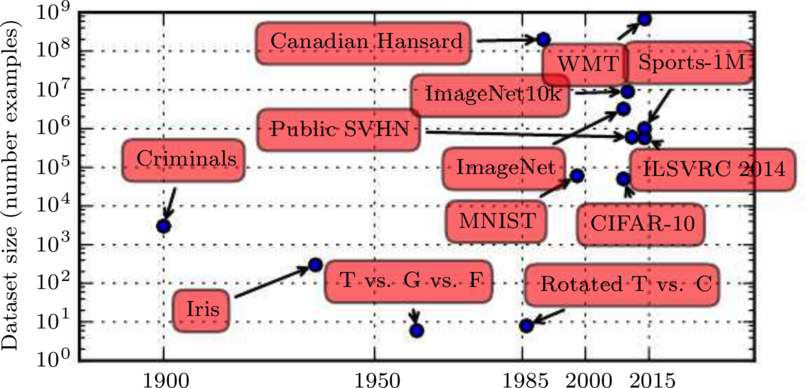
\includegraphics[scale=0.5]{images/8.png}}
\else
\centerline{\includegraphics{Chapter1/figures/dataset_size_color}}
\fi
\caption{与日俱增的数据量。
20世纪初,统计学家使用数百或数千的手动制作的度量来研究数据集\citep{Garson-1900,Gosset-1908,Anderson-1935,Fisher-1936}。
20世纪50年代到80年代,受生物启发的机器学习开拓者通常使用小的合成数据集,如低分辨率的字母位图,设计为在低计算成本下表明神经网络能够学习特定功能\citep{Widrow-Hoff-1960,Rumelhart-et-al-1986b}。
20世纪80年代和90年代,机器学习变得更加统计,并开始利用包含成千上万个样本的更大数据集,如手写扫描数字的MNIST数据集(如\figref{fig:chap1_mnist})所示\citep{LeCun-et-al-1998b}。
在21世纪初的第一个十年,相同大小更复杂的数据集持续出现,如CIFAR-10数据集\citep{Krizhevsky-Hinton-2009} 。
在这十年结束和下五年,明显更大的数据集(包含数万到数千万的样例)完全改变了深度学习的可能实现的事。
这些数据集包括公共Street View House Numbers数据集 \citep{Netzer-et-al-2011}、各种版本的ImageNet数据集\citep{Deng-et-al-2009,Deng-et-al-2010a,Russakovsky-et-al-2014a}以及Sports-1M数据集\citep{Karpathy-et-al-2014}。
在图顶部,我们看到翻译句子的数据集通常远大于其他数据集,如根据Canadian Hansard制作的IBM数据集\citep{Brown-et-al-1990}和WMT 2014英法数据集\citep{Schwenk-2014} 。
}
\label{fig:chap1_dataset_size_color}
\end{figure}
\begin{figure}[!htb]
\ifOpenSource
\centerline{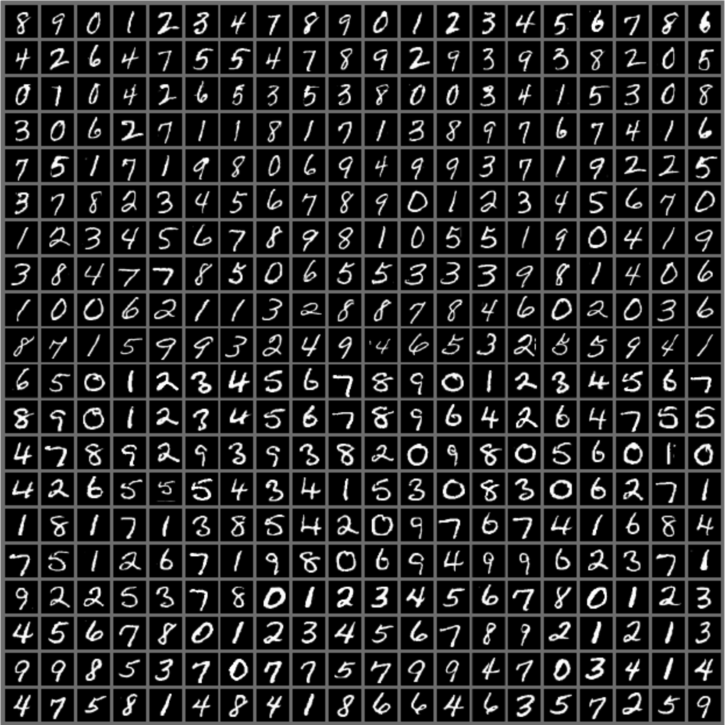
\includegraphics[scale=0.5]{images/9.png}}
\else
\centerline{\includegraphics[width=0.8\textwidth]{Chapter1/figures/mnist}}
\fi
\caption{MNIST数据集的输入样例。
``NIST''代表国家标准和技术研究所(National Institute of Standards and Technology),是最初收集这些数据的机构。
``M''代表``修改的(Modified)'',为更容易地与机器学习算法一起使用,数据已经过预处理。
MNIST数据集包括手写数字的扫描和相关标签(描述每个图像中包含0-9中哪个数字)。
这个简单的分类问题是深度学习研究中最简单和最广泛使用的测试之一。
尽管现代技术很容易解决这个问题,它仍然很受欢迎。
Geoffrey Hinton将其描述为``机器学习的\emph{果蝇}'',这意味着机器学习研究人员可以在受控的实验室条件下研究他们的算法,就像生物学家经常研究果蝇一样。
}
\label{fig:chap1_mnist}
\end{figure}

% -- 20 --

\subsection{与日俱增的模型规模}
\label{sec:increasing_model_sizes}


20世纪80年代,\gls{NN}只能取得相对较小的成功,而现在\gls{NN}非常成功的另一个重要原因是我们现在拥有的计算资源可以运行更大的模型。
\gls{connectionism}的主要见解之一是,当动物的许多神经元一起工作时会变得聪明。
单独神经元或小集合的神经元不是特别有用。

生物神经元不是特别稠密地连接在一起。
如\figref{fig:chap1_number_of_synapses_color}所示,几十年来,我们的\gls{ML}模型中每个神经元的连接数量已经与哺乳动物的大脑在同一数量级上。

\begin{figure}[!htb]
\ifOpenSource
\centerline{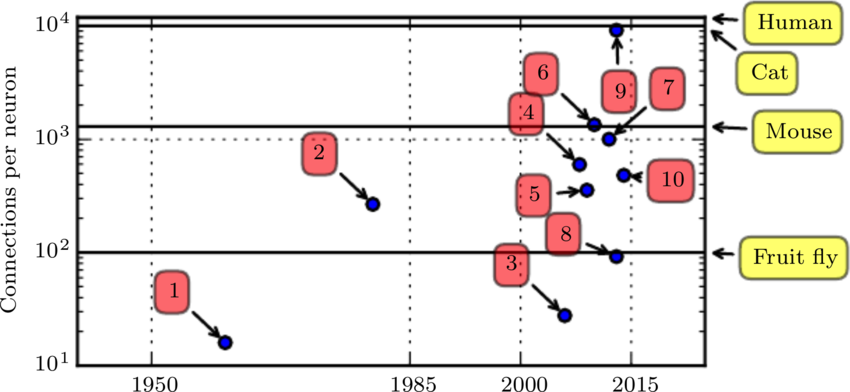
\includegraphics[scale=0.5]{images/10.png}}
\else
\centerline{\includegraphics{Chapter1/figures/number_of_synapses_color}}
\fi
\caption{与日俱增的每神经元连接数。 % ? 可以翻成平均吗 ?
最初,\gls{ANN}中神经元之间的连接数受限于硬件能力。
而现在,神经元之间的连接数大多是出于设计考虑。
一些\gls{ANN}中每个神经元的连接数与猫一样多,并且对于其他神经网络来说,每个神经元的连接与较小哺乳动物(如小鼠)一样多是非常普遍的。
甚至人类大脑每个神经元的连接也没有过高的数量。
生物神经网络规模来自\citet{Wikipedia-2015}。
}
\label{fig:chap1_number_of_synapses_color}
{\tiny
\begin{enumerate}
  \itemsep0em
  \item % 1
    自适应线性单元~\citep{Widrow-Hoff-1960}
  \item % 2
    神经认知机~\citep{Fukushima-1980}
  \item % 3
    GPU-加速 \gls{convolutional_network}~\citep{Chellapilla-et-al-2006}
  \item % 4
    \gls{DBM}~\citep{Salakhutdinov-Hinton-2009a}
  \item % 5
    \gls{unsupervised}\gls{convolutional_network}~\citep{Jarrett-et-al-2009}
  \item % 6
    GPU-加速 \gls{MLP}~\citep{Ciresan-et-al-2010}
  \item % 7
    分布式\gls{AE}~\citep{Le-et-al-2012}
  \item % 8
    Multi-GPU \gls{convolutional_network}~\citep{Krizhevsky-et-al-2012}
  \item % 9
    COTS HPC  \gls{unsupervised}\gls{convolutional_network}~\citep{Coates-et-al-2013}
  \item % 10
    GoogLeNet~\citep{Szegedy-et-al-2014a}
\end{enumerate}
} % end tiny
\end{figure}

如\figref{fig:chap1_number_of_neurons_color}所示,就神经元的总数目而言,直到最近\gls{NN}都是惊人的小。
自从\gls{hidden_unit}引入以来,人工\gls{NN}的规模大约每2.4年扩大一倍。
这种增长是由更大内存、更快的计算机和更大的可用数据集驱动的。
更大的网络能够在更复杂的任务中实现更高的精度。
这种趋势看起来将持续数十年。
除非有能力迅速扩展的新技术,否则至少要到21世纪50年代,人工\gls{NN}将才能具备与人脑相同数量级的神经元。
生物神经元表示的功能可能比目前的人工神经元所表示的更复杂,因此生物神经网络可能比图中描绘的甚至要更大。

\begin{figure}[!htb]
\ifOpenSource
\centerline{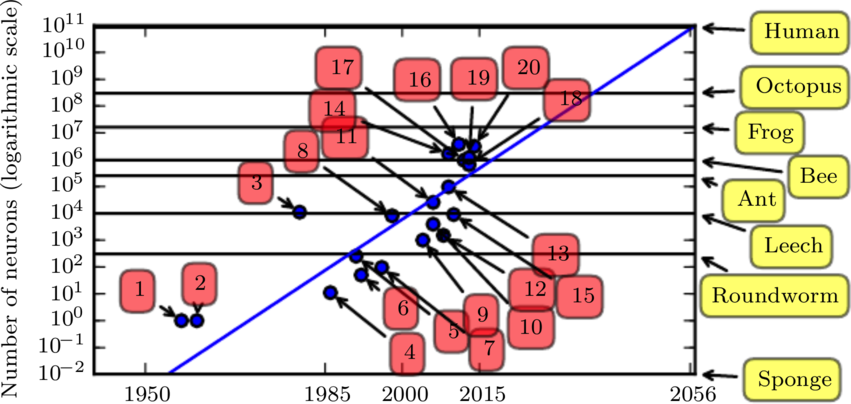
\includegraphics[scale=0.5]{images/11.png}}
\else
\centerline{\includegraphics{Chapter1/figures/number_of_neurons_color}}
\fi
\caption{与日俱增的神经网络规模。
自从引入\gls{hidden_unit},\gls{ANN}的大小大约每2.4年翻一倍。
生物神经网络规模来自~\citet{Wikipedia-2015}。
}
\label{fig:chap1_number_of_neurons_color}
{\tiny
\begin{enumerate}
  \itemsep-.1em
  \item % 1
    感知机~\citep{Rosenblatt-1958,Rosenblatt-1962}
  \item % 2
    自适应线性单元~\citep{Widrow-Hoff-1960}
  \item % 3
    神经认知机~\citep{Fukushima-1980}
  \item % 4
    早期后向传播网络~\citep{Rumelhart-et-al-1986b}
  \item % 5
    用于语音识别的\gls{RNN}~\citep{Robinson-Fallside-1991}
  \item % 6
    用于语音识别的\gls{MLP}~\citep{Bengio-et-al-1991}
  \item % 7
    \gls{meanfield}sigmoid\gls{BN}~\citep{Saul-et-al-1996}
  \item % 8
    LeNet-5~\citep{LeCun-et-al-1998b}
  \item % 9
    \gls{ESN}~\citep{Jaeger-Haas-2004}
  \item % 10
    \gls{DBN}~\citep{Hinton-et-al-2006}
  \item % 11
    GPU-加速\gls{convolutional_network}~\citep{Chellapilla-et-al-2006}
  \item % 12
    \gls{DBM}~\citep{Salakhutdinov-Hinton-2009a}
  \item % 13
    GPU-加速\gls{DBN}~\citep{Raina-et-al-2009}
  \item % 14
    \gls{unsupervised}\gls{convolutional_network}~\citep{Jarrett-et-al-2009}
  \item % 15
    GPU-加速\gls{MLP}~\citep{Ciresan-et-al-2010}
  \item % 16
    OMP-1 网络~\citep{Coates-Ng-2011}
  \item % 17
    分布式\gls{AE}~\citep{Le-et-al-2012}
  \item % 18
    Multi-GPU\gls{convolutional_network}~\citep{Krizhevsky-et-al-2012}
  \item % 19
    COTS HPC \gls{unsupervised}\gls{convolutional_network}~\citep{Coates-et-al-2013}
  \item % 20
    GoogLeNet~\citep{Szegedy-et-al-2014a}
\end{enumerate}
}
\end{figure}


现在看来,其神经元比一个水蛭还少的\gls{NN}不能解决复杂的\gls{AI}问题是不足为奇的。
即使现在的网络,从计算系统角度来看它可能相当大的,但实际上它比相对原始的脊椎动物如青蛙的神经系统还要小。

由于更快的CPU、通用GPU的出现(在\secref{sec:gpu_implementations}中讨论)、更快的网络连接和更好的分布式计算的软件基础设施,模型规模随着时间的推移不断增加是\gls{DL}历史中最重要的趋势之一。
人们普遍预计这种趋势将很好地持续到未来。

% -- 21 --

\subsection{与日俱增的精度、复杂度和对现实世界的冲击}
\label{sec:increasing_accuracy_complexity_and_real_world_impact}

20世纪80年代以来,\gls{DL}提供精确识别和预测的能力一直在提高。
而且,\gls{DL}持续成功地被应用于越来越广泛的实际问题中。

最早的深度模型被用来识别裁剪紧凑且非常小的图像中的单个对象\citep{Rumelhart-et-al-1986a}。
此后,\gls{NN}可以处理的图像尺寸逐渐增加。
现代对象识别网络能处理丰富的高分辨率照片,并且不需要在被识别的对象附近进行裁剪\citep{Krizhevsky-et-al-2012}。
类似地,最早的网络只能识别两种对象(或在某些情况下,单类对象的存在与否),而这些现代网络通常能够识别至少\NUMTEXT{1000}个不同类别的对象。
对象识别中最大的比赛是每年举行的ImageNet大型视觉识别挑战(ILSVRC)。
\gls{DL}迅速崛起的激动人心的一幕是卷积网络第一次大幅赢得这一挑战,它将最高水准的前5错误率从~\NUMTEXT{26.1\%}~降到~\NUMTEXT{15.3\%}~\citep{Krizhevsky-et-al-2012},这意味着该卷积网络针对每个图像的可能类别生成一个顺序列表,除了15.3\%的测试样本,其他测试样本的正确类标都出现在此列表中的前5项里。
此后,深度卷积网络连续地赢得这些比赛,截至写本书时,\gls{DL}的最新结果将这个比赛中的前5错误率降到了~\NUMTEXT{3.6\%}, 如\figref{fig:chap1_imagenet_color}所示。

\begin{figure}[!htb]
\ifOpenSource
\centerline{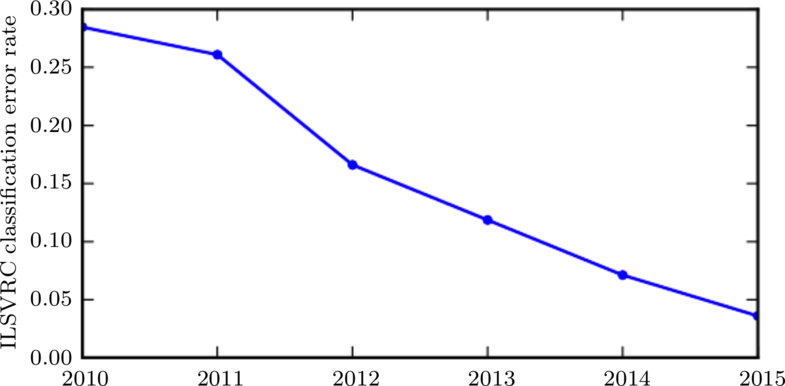
\includegraphics[scale=0.5]{images/12.png}}
\else
\centerline{\includegraphics{Chapter1/figures/imagenet_color}}
\fi
\caption{日益降低的错误率。
由于深度网络达到了在ImageNet大规模视觉识别挑战中竞争所必需的规模,它们每年都能赢得胜利,并且产生越来越低的错误率。
数据来源于 \citet{Russakovsky-et-al-2014a}和~\citet{He-et-al-2015}。}
\label{fig:chap1_imagenet_color}
\end{figure}

% -- 23 --

\gls{DL}也对语音识别产生了巨大影响。
语音识别在20世纪90年代得到提高后,直到约2000年都停滞不前。
\gls{DL}的引入\citep{Dahl-et-al-2010,Deng-et-al-2010b,Seide-et-al-2011,Hinton-et-al-2012a}使得语音识别错误率陡然下降,有些错误率甚至降低了一半。
我们将在\secref{sec:speech_recognition}更详细地探讨这个历史。

深度网络在行人检测和图像分割中也取得了引人注目的成功\citep{Sermanet-et-al-2013,Farabet-et-al-2013,Couprie-et-al-2013},并且在交通标志分类上取得了超越人类的表现\citep{Ciresan-et-al-2012}。

在深度网络的规模和精度有所提高的同时,它们可以解决的任务也日益复杂。
\citet{Goodfellow-et-al-2014d}表明,\gls{NN}可以学习输出描述图像的整个字符序列,而不是仅仅识别单个对象。
此前,人们普遍认为,这种学习需要对序列中的单个元素进行标注\citep{Gulcehre-Bengio-2013}。
\gls{RNN},如之前提到的~\glssymbol{LSTM}~序列模型,现在用于对序列和其他序列之间的关系进行建模,而不是仅仅固定输入之间的关系。
这种序列到序列的学习似乎引领着另一个应用的颠覆性发展,即机器翻译\citep{Sutskever-et-al-2014,Bahdanau-et-al-2015}。

% -- 24 --

这种复杂性日益增加的趋势已将其推向逻辑结论,即神经图灵机\citep{Graves-et-al-2014a}的引入,它能学习读取存储单元和向存储单元写入任意内容。
这样的\gls{NN}可以从期望行为的\gls{example}中学习简单的程序。
例如,从杂乱和排好序的\gls{example}中学习对一系列数进行排序。
这种自我编程技术正处于起步阶段,但原则上未来可以适用于几乎所有的任务。


\gls{DL}的另一个最大的成就是其在\firstgls{RL}领域的扩展。
在\gls{RL}中,一个自主的智能体必须在没有人类操作者指导的情况下,通过试错来学习执行任务。
DeepMind表明,基于\gls{DL}的\gls{RL}系统能够学会玩Atari视频游戏,并在多种任务中可与人类匹敌\citep{Mnih-et-al-2015}。
\gls{DL}也显著改善了机器人\gls{RL}的性能\citep{Finn-et-al-2015}。

许多\gls{DL}应用都是高利润的。现在\gls{DL}被许多顶级的技术公司使用,包括Google、Microsoft、Facebook、IBM、Baidu、Apple、Adobe、Netflix、NVIDIA和NEC等。

\gls{DL}的进步也严重依赖于软件基础架构的进展。
软件库如Theano~\citep{Bergstra-et-al-2010,Bastien-et-al-2012}、PyLearn2~\citep{Goodfellow-et-al-2013c}、Torch~\citep{Collobert-et-al-2011b}、DistBelief~\citep{Dean-et-al-2012}、Caffe~\citep{Jia-2013}、MXNet~\citep{Chen-et-al-2015}和TensorFlow~\citep{Abadi-et-al-2015}都能支持重要的研究项目或商业产品。

\gls{DL}也为其他科学做出了贡献。
用于对象识别的现代卷积网络为神经科学家们提供了可以研究的视觉处理模型\citep{DiCarlo-2013}。
\gls{DL}也为处理海量数据以及在科学领域作出有效的预测提供了非常有用的工具。
它已成功地用于预测分子如何相互作用从而帮助制药公司设计新的药物\citep{Dahl-et-al-2014},搜索亚原子粒子\citep{Baldi-et-al-2014},以及自动解析用于构建人脑三维图的显微镜图像\citep{KnowlesBarley-et-al-2014}等。
我们期待\gls{DL}未来能够出现在越来越多的科学领域中。

% -- 25 --

总之,\gls{DL}是\gls{ML}的一种方法。在过去几十年的发展中,它大量借鉴了我们关于人脑、统计学和应用数学的知识。
近年来,得益于更强大的计算机、更大的数据集和能够训练更深网络的技术,\gls{DL}的普及性和实用性都有了极大的发展。
未来几年充满了进一步提高\gls{DL}并将它带到新领域的挑战和机遇。

% -- 26 --
